\section{Hardware and setup} \label{hardware}

\subsection{Raytrix Technology}\label{the_raytrix_camera}

\begin{figure}[ht]
    \centering
    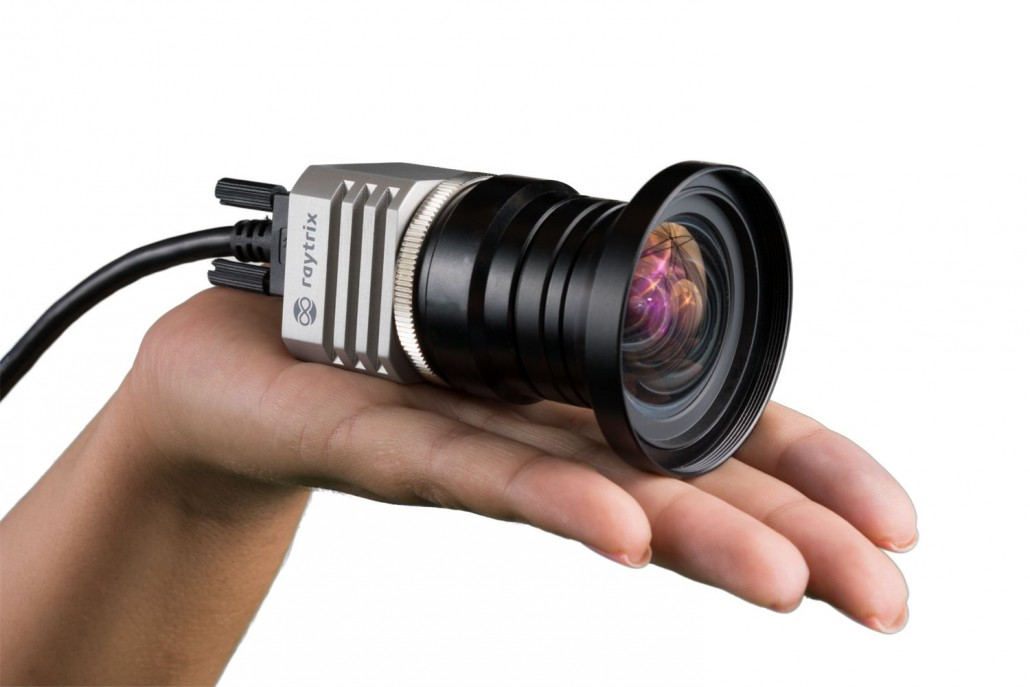
\includegraphics[width=.9\linewidth]{images/hardware/raytrix_camera}
    \caption{Raytrix R42 Camera\cite{website:raytrix_r42}}
    \label{fig:raytrix_camera}
\end{figure}

The camera used throughout this project is the Raytrix R42 camera. The camera is developed by Raytrix, a German company which offers several 3D Light Field cameras intended for professional and industrial use. The R42 is their highest resolving light field camera to date. It is based on a 42 megaray sensor and offers an effective resolution up to 10 megapixels at 7 FPS. \cite{website:raytrix_r42}

Light Field cameras are a new type of 3D-cameras that capture both a standard image and the depth information of a scene. Metric 3D information can be captured with a single light field camera through a single lens in a single shot using just the available light. Raytrix has specialized on light field cameras for industrial use. The Raytrix micro lens array design allows for an optimal compromise between high effective resolution and large depth of field. Raytrix cameras are already in use in applications like volumetric velocimetry, plant phenotyping, automated optical inspection and microscopy, to name a few. \cite{website:raytrix_main}

The Raytrix camera contains of a main lens in front, a micro lens array in the middle, and the image sensor behind. The micro lens array has many thousand micro lenses, about 4000 lenses. The micro lens array is placed in front of the image sensor inside the camera, which turns the image sensor into a micro-camera array (see figure \ref{fig:light_field}), where each micro-camera sees part of the intermediate image from a slightly different perspective. That is, instead of using a large camera array that looks directly at the object, it is possible to choose a main lens to select the desired field-of-view and create the intermediate image in front of the micro camera array. A narrower field-of-view makes more micro lenses see each small part of the object, and makes for more accurate 3D-images. The images generated by the camera in this setup are processed on a PC with appropriate software algorithms to calculate the scene depth and to reconstruct a 2D image. When all processing is done on a GPU, it allows for high resolution 2D and 3D images, at up to 7 FPS. \cite{website:raytrix_technology}

\begin{figure}[h]
    \centering
    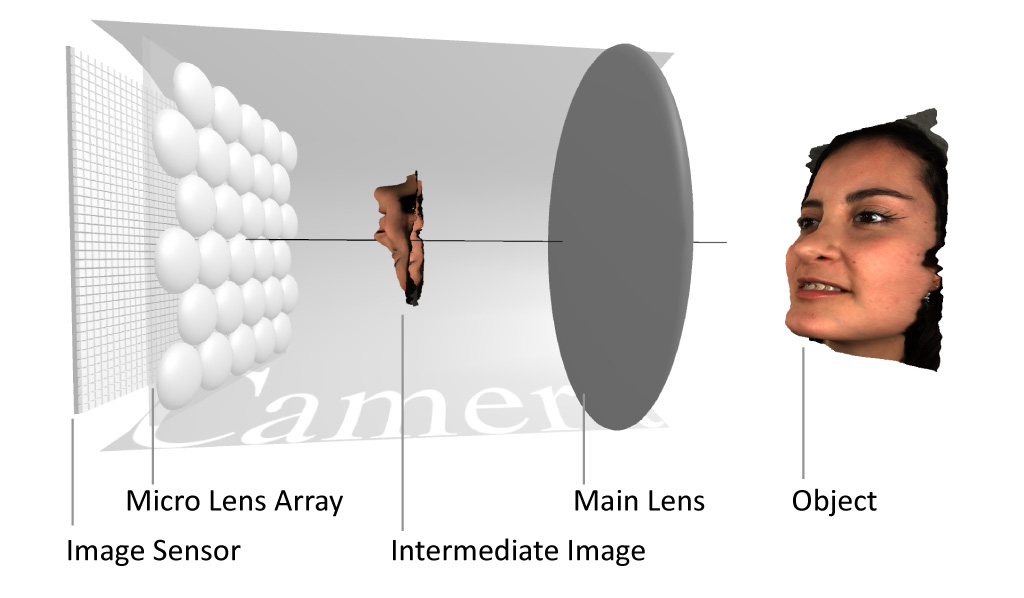
\includegraphics[width=.9\linewidth]{images/hardware/Light-Field-Camera-Schematic}
    \caption{Raytrix Light Field Technology\cite{website:raytrix_technology}}
    \label{fig:light_field}
\end{figure}

When calibrating the camera the raw image is used to make sure the main objects edges are shown in several of the micro lenses. The more micro lenses picking up each small part of the object, the more accurate the depth information. 

The raw image shows the capture from all micro lenses, as seen in figure \ref{fig:raw_image}. It is seen that the straight edges is shown in several micro lenses. The camera perform no processing internally, it simply deliver the raw image to a PC, which is then processed on a GPU to obtain the 2D and 3D data. 
The totalfocus image is a 2D image using all focus information from each individual micro lens to compute an image. This is made from the raw image and the 3D data on a computer, and will be an image with the whole frame as focus area, see figure \ref{fig:totalfocus}. 
Raytrix also computes a refocus image, that uses the raw image and the 3D data to compute an image with the desired area in focus. This focus area can be moved around after image taking.
Figure \ref{fig:3d_image} shows the 3D image in the Raytrix software. This is made from the 3D information and the totalfocus image. 
The depthmap, figure \ref{fig:depthmap}, is computed from the the 3D information, and is a color image where each color represents a depth. The depth for each color is determined by the calibration data and depends on the chosen distance to the object and more. 
Red is close to the camera, yellow and green is the object centered during calibration, blue is behind the object, and black is beyond the distance set during calibration.


\begin{figure}[h]
    \begin{subfigure}{0.49\textwidth}
        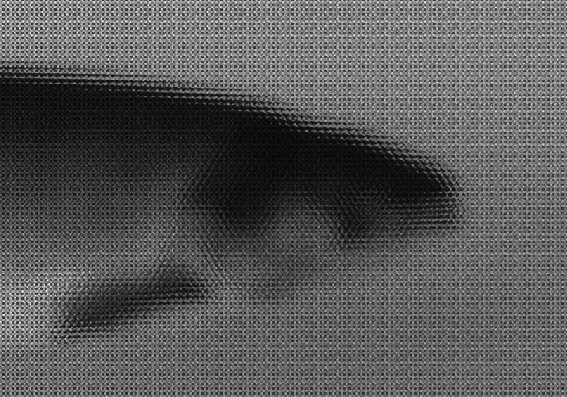
\includegraphics[width=\linewidth]{images/hardware/raytrix_raw_image}
        \caption{Raw image} 
        \label{fig:raw_image}
    \end{subfigure}\hspace*{\fill}
    \begin{subfigure}{0.49\textwidth}
        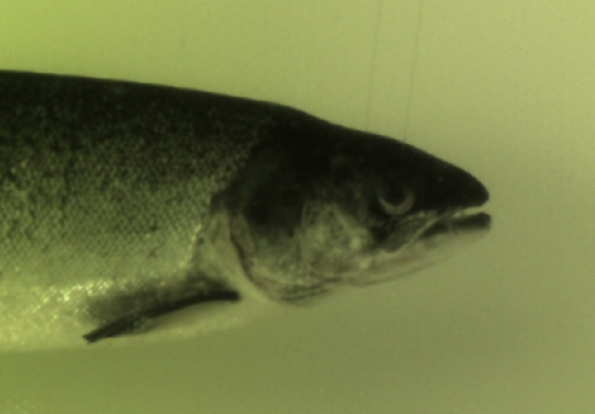
\includegraphics[width=\linewidth]{images/hardware/raytrix_totalfocus_image}
        \caption{Totalfocus image} 
        \label{fig:totalfocus}
    \end{subfigure}
    
    \medskip
    \begin{subfigure}{0.49\textwidth}
        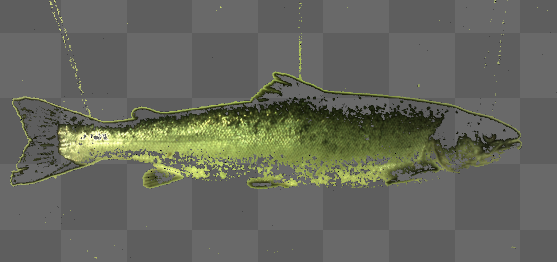
\includegraphics[width=\linewidth]{images/hardware/raytrix_3D_image}
        \caption{3D image} 
        \label{fig:3d_image}
    \end{subfigure}\hspace*{\fill}
    \begin{subfigure}{0.49\textwidth}
        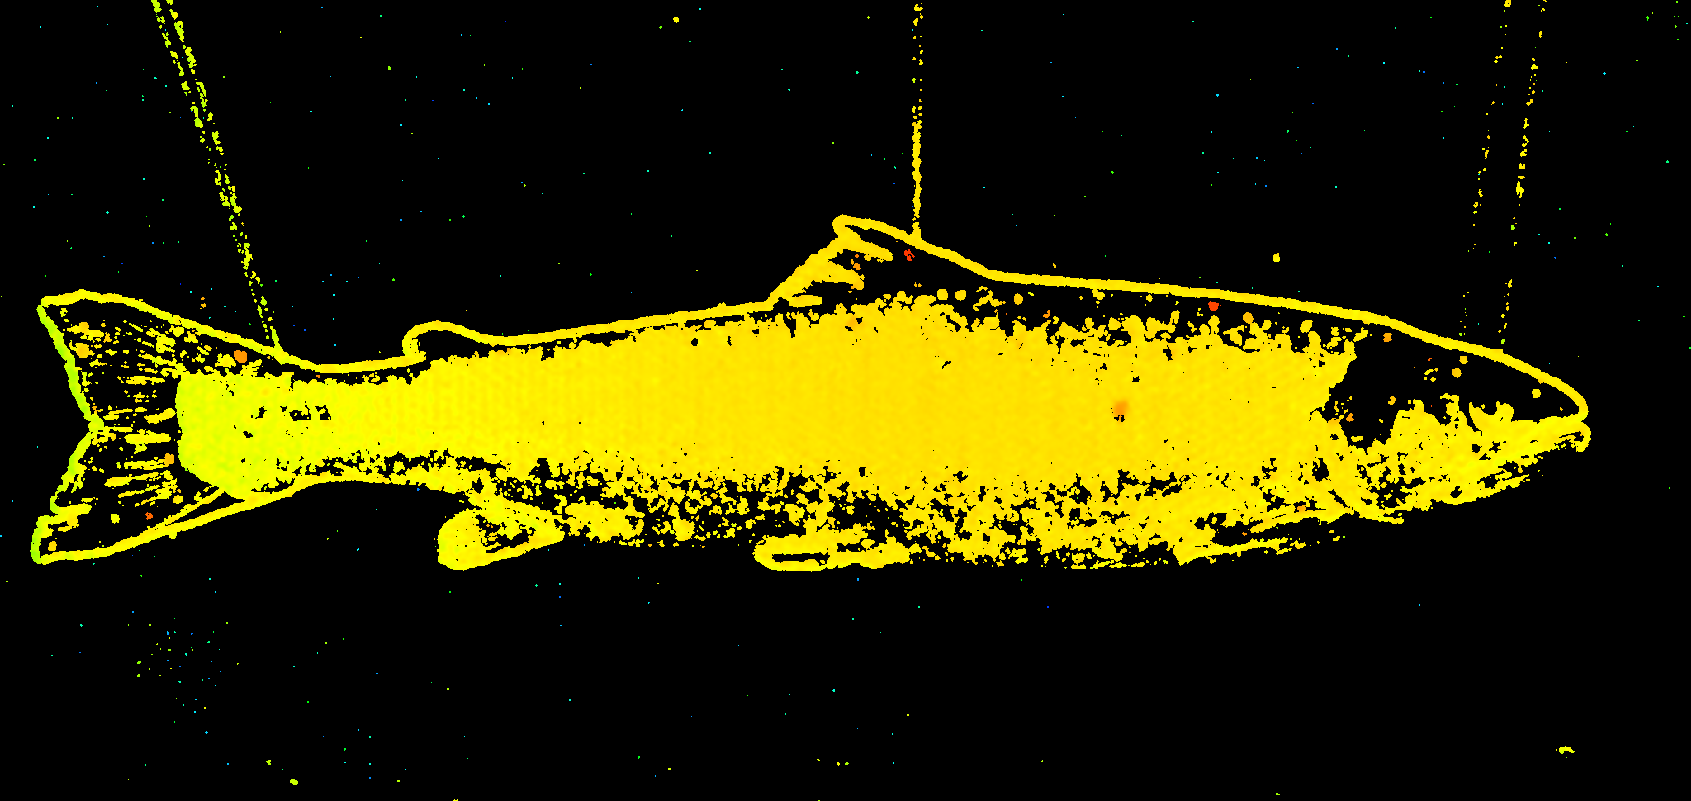
\includegraphics[width=\linewidth]{images/hardware/raytrix_depthmap_image}
        \caption{Depthmap image} 
        \label{fig:depthmap}
    \end{subfigure}
    \caption{Images computed by the Raytrix} 
    \label{fig:raytrix_captures}
\end{figure}

As seen from the 3D image produced in the Raytrix Software, the particles in front will affect the surface of the object. The same goes for holes in the object. As seen from the MATLAB 3D-model in figure \ref{fig:matlab3D}, there is large disturbances in the computed 3D image.

The reason the Raytrix R42 camera is used is because of its high resolution and high frame-rate, which non of Raytrix's competitors can match. The Raytrix camera is also different from other light field cameras because it has the light ray crossing behind the micro lens array, while other light field cameras have the light crossing in front of the micro lens array.\cite{article:stereo_vs_plenoptic}

One problem working with the Raytrix is that the depth information is stored in their own .ray format. It is not yet possible to do direct image processing on this format using other processing tools than Raytrix's own software, RxLive. RxLive has some good software tools, but to do more advanced image processing the software is not sufficient.
Another problem is the calibration of the Raytrix. For every time the camera is calibrated the colors in the depthmap, representing the depth, change. If image processing on the depthmap is to be the solution, a way of incorporating the depth data into the depthmap must be found.

All images in this subsection is made with the Raytrix software, RxLive 4.0.


%%%%%%%%%%%%%%%%%%%%%%%%%%%%%%%%%%%%%%%%%%%%%%%%%%%%%%%%%%%%%%%%%%%%%%


\subsection{Wetlab}\label{wetlab}

SEALAB OCEAN GROUP has its own test facility with a small fish tank with setup for different cameras and lights. The wetlab have setup for both the Raytrix R42, a Sony 2D camera for high resolution images and underwater lights. The cameras are directly connected to computers, so it is possible to work remotely.

SEALAB have an agreement with Marine Harvest so it is possible to get fish delivered to the wetlab for testing.

The fish tank was originally white, but during a period with testing it was painted black so the background would imitate the open ocean. Figure \ref{fig:wetlab} gives a clearer picture of the wetlab.

\begin{figure}[h]
    \centering
    \begin{subfigure}{1\textwidth}
        \centering
        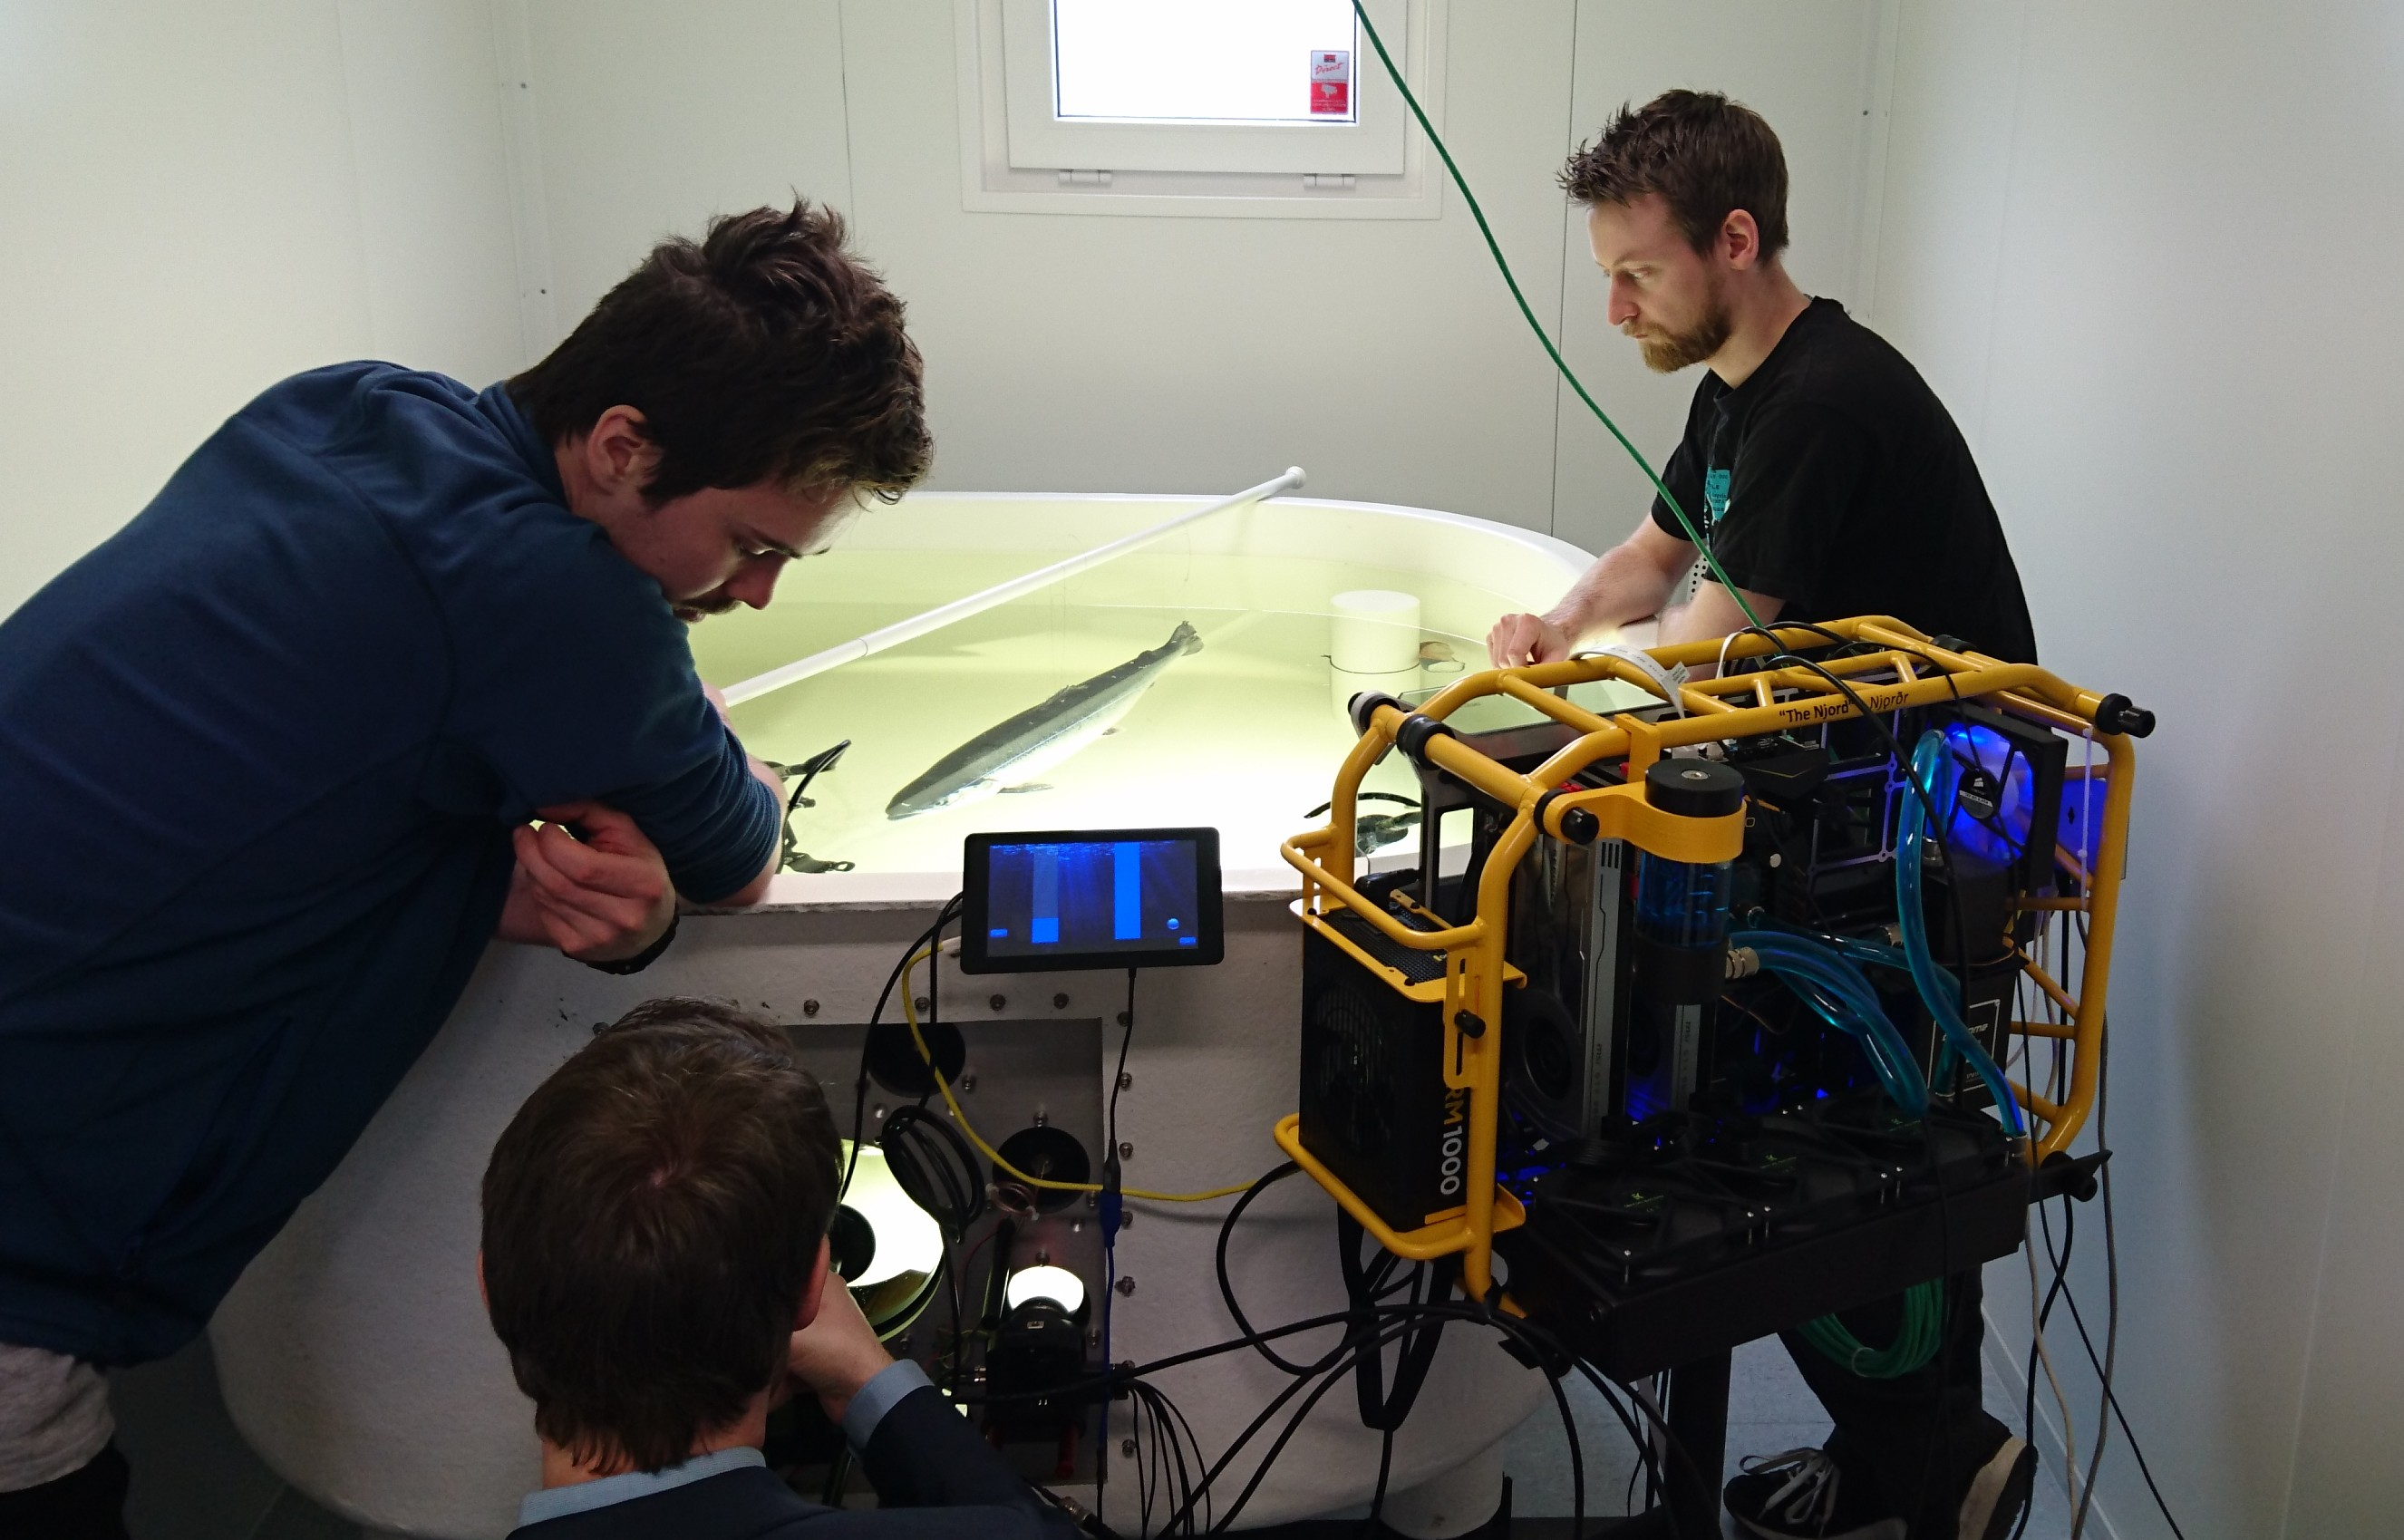
\includegraphics[width=.6\linewidth]{images/hardware/wetlab_overview}
        \caption{Test facility} 
    \end{subfigure}\hspace*{\fill}
    
    \medskip
    \begin{subfigure}{1\textwidth}
        \centering
        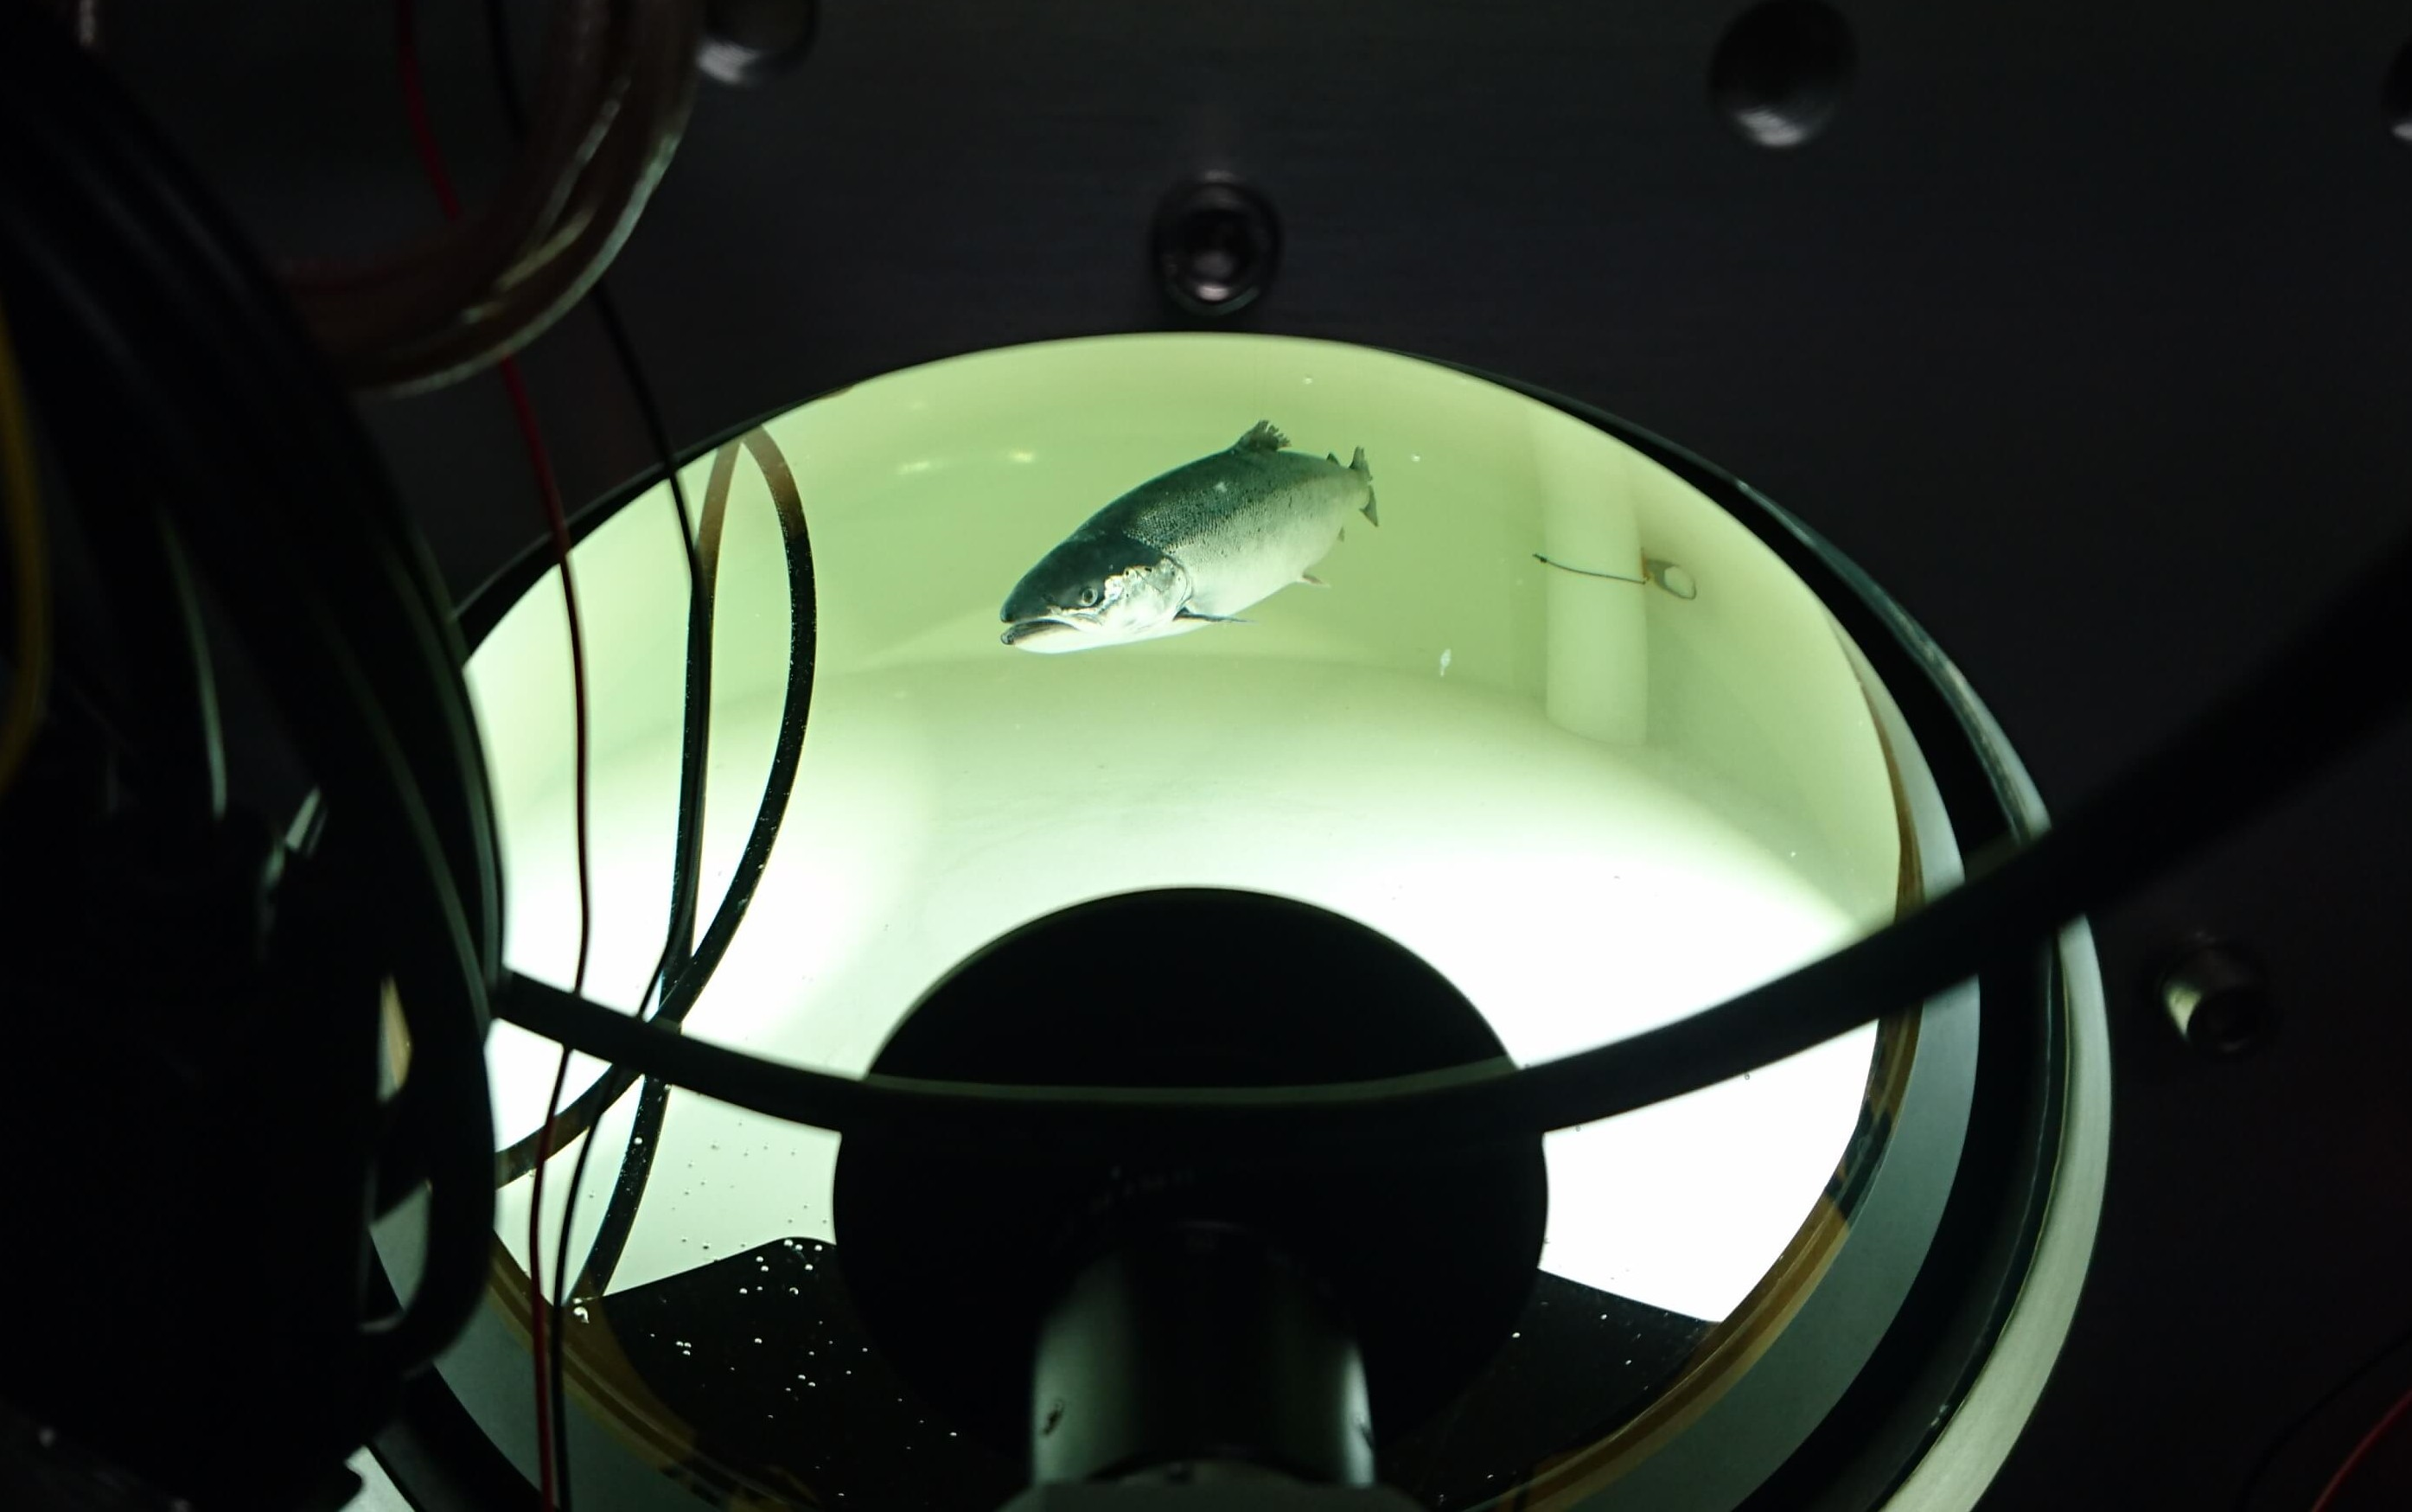
\includegraphics[width=.6\linewidth]{images/hardware/wetlab_fish_dome}
        \caption{Raytrix view with white background} 
    \end{subfigure}\hspace*{\fill}
    
    \medskip
    \begin{subfigure}{1\textwidth}
        \centering
        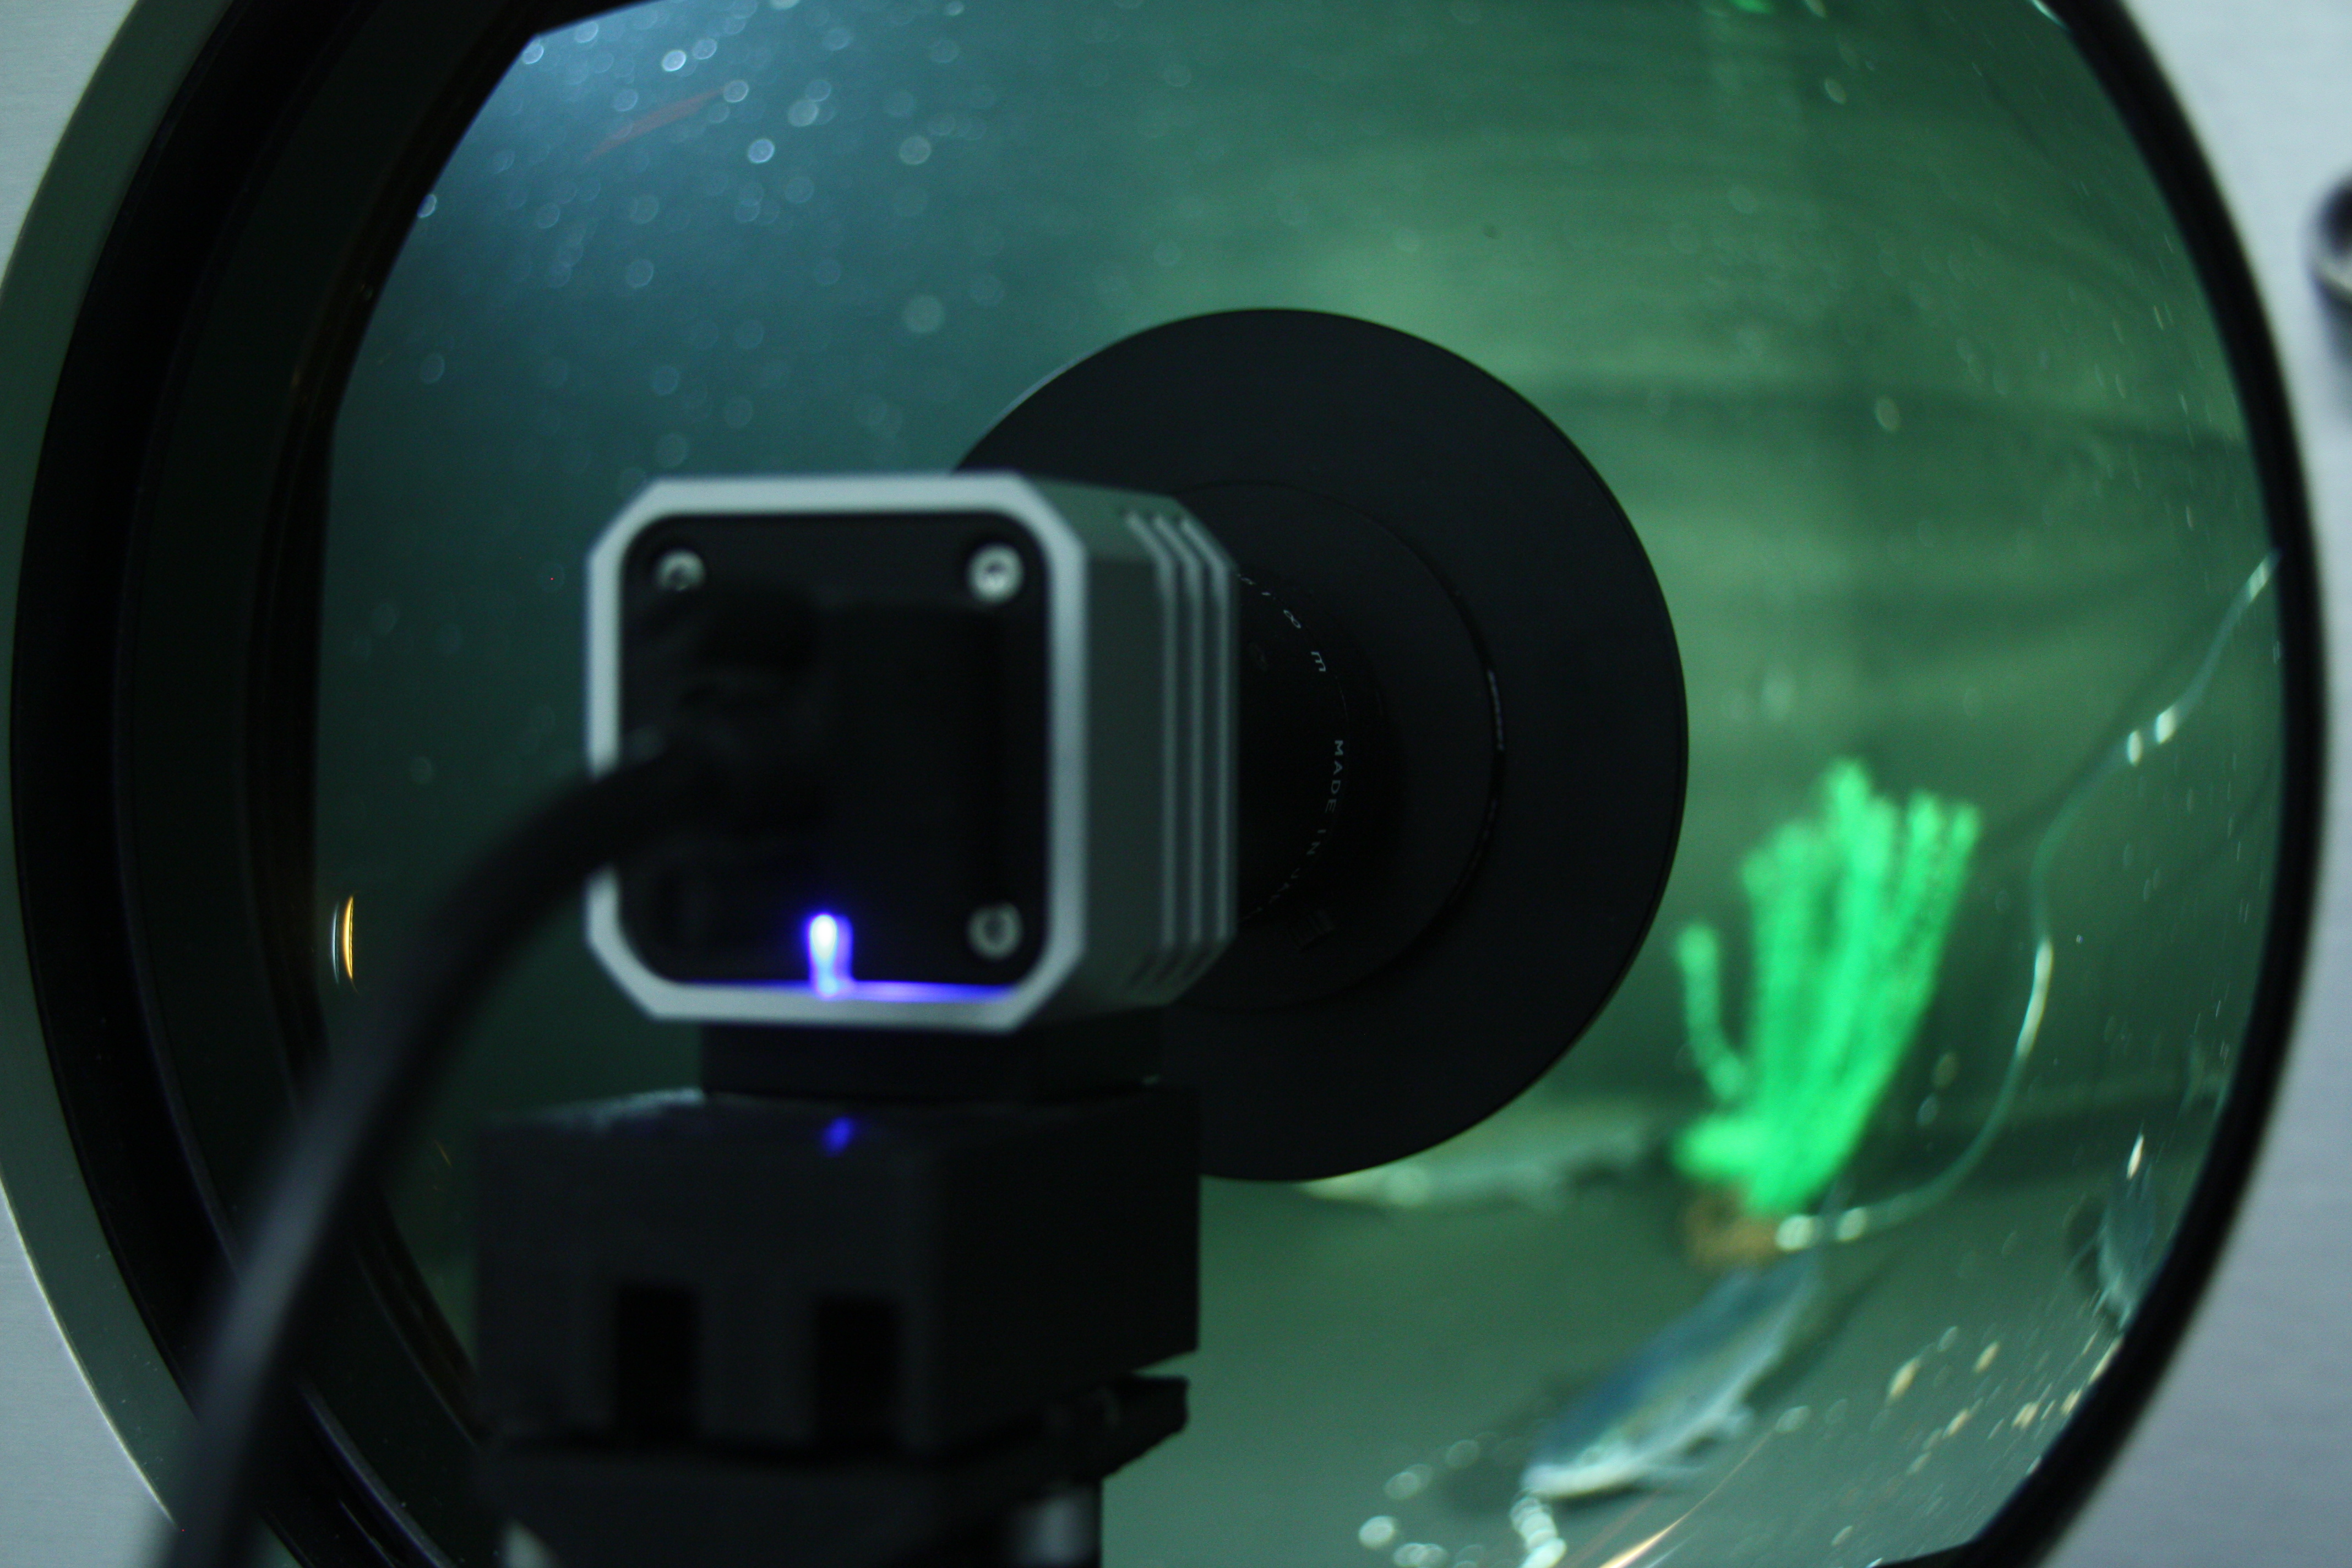
\includegraphics[width=.6\linewidth]{images/hardware/wetlab_raytrix}
        \caption{Raytrix view with black background} 
    \end{subfigure}\hspace*{\fill}
    \caption{Wetlab \cite{website:sealab}}
    \label{fig:wetlab}
\end{figure}









